
% Zitat ?

This chapter will give an implementation of \algo
that cannot make use of NDP. This is
the case when one is only given a few parallel primitives
that don't support nesting
of operations (at least not without falling back to sequential evaluation).
Table \ref{table:parprims} shows a few of these primitives.

  \begin{table}[h!]
    \caption{Parallel Primitives in Flat Data Parallelism}
    \label{table:parprims}
    \begin{center}
    \begin{tabular}{lll}
      \toprule
      function & type \\
      \midrule
      parMap & \c{(a -> b) -> Vector a -> Vector b} \\
      parZipWith & \c{(a -> b -> c)} \\
       & \c{Vector a -> Vector b -> Vector c} \\
      parReplicate & \c{Int -> a -> Vector a} \\
      parGenerate & \c{Int -> (Int -> a) -> Vector a} \\
    \end{tabular}
    \end{center}
  \end{table}
  They are analogous to the parallel functions in NDP.
  \c{parGenerate} is a function such that \c{parGenerate size f} creates a new array
  of size \c{size} and uses the generator function \c{f} to create
  the elements by their indices.
  E.g. \c{parGenerate 5 (\lam i -> i*i) = [0,1,4,9,16] }.
  These primitives all have work $O(n)$ and depth $O(1)$.
  
\section{Parallel histogram accumulation}
  To implement \algo in parallel, one has to revisit the sequential
  implementation. The parallel creation of the accumulated histogram is
  a difficult task. The goal is to try to come up with
  an low complexity algorithm for the histogram calcuation.
  After a few tries, one can give the following implementation:
  
  \begin{lstlisting}
accuHist :: Image -> Hist
accuHist []  = parReplicate gmax 0
accuHist [x] = parGenerate gmax (\i -> if (i >= x) then 1 else 0)
accuHist xs  = let (left,right) = splitMid xs
                   [leftRes,rightRes] = parMap accuHist [left,right]
               in  parZipWith (+) leftRes rightRes
  \end{lstlisting}
  The general idea is to merge accumulation and histogram creation
  into a single tree-like reduction. To each array of pixels, \c{accuHist}
  returns the accumulated histogram of its gray tones.
  The algorithim can be broken down into two edge-cases and one recursive case
  . Figure \ref{figure:accuHist} gives an example of its evaluation.
  
  \begin{figure}[h]
    \centering
    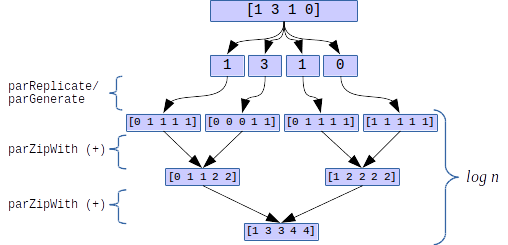
\includegraphics[width=\linewidth]{accuHist}
    \label{figure:accuHist}
    \caption{Evaluation of \c{accuHist [1,3,1,0]}}
  \end{figure}
  
  Suppose \c{gmax = 4} then the algorithm returns \c{[0 0 0 0 0]} if
  the input array was empty. If the image only contained a single gray tone
  \c{x}, then it creates its accumulated histogram
  \c{[0 0 ... 0 1 ... 1 1]} such that \c{x} is the index
  of the first \c{1}.
  For example, for \c{x = 2} the array
  \c{[0 0 1 1 1]} is returned. This is implemented using the \c{parGenerate} function.
  Finally, one has the recursive case. In this case, the the calculation
  of larger images is broken down by splitting the array into half
  \footnote{splitting is a constant time operation
  for these view-based arrays} and applying \c{accuHist}
  recursively. Finally, the histograms are merged with elementwise addition
  ({\c{zipWith(+)}}).
  
  This algorithm was carefully constructed after many failed approaches
  on such an algorithm. Alternatives were considered, but they did not
  yield an acceptable complexity compared to \c{accuHist}.

\section{Implementation}
  Given the introduction, the manurally parallised \man can finally be implemented.
  The parallel primitives can be integrated
  well into normalisation and scaling.
  However, \c{accuHist} and \c{apply} need to be adapted.
  The code is given below. \c{(!)} is used for indexing.
  \begin{lstlisting}
type Image  = Vector Int
type Hist   = Vector Int

hbalance :: Image -> Image
hbalance img =
  let hist = accuHist img
      a0 = hist ! 0
      agmax = hist ! gmax
      apply gs = parMap (\i -> gs ! i) img
      sclNrm :: Int -> Int
      sclNrm x = floor ( (x-a0)/(agmax - a0)*gmax )
  in  apply (parMap sclNrm) hist
  \end{lstlisting}
  As explained in the previous section, the parallel
  accumulated histogram calculation has been implemented in \c{accuHist}.
  For the gray tone mapping (\c{apply}) to work, nested arrays cannot be used
  \footnote{as they would result into an array of pointers to subarrays.
  This is undesireable due to Cache Locality.}
  .
  One needs to change the entire image representation to a flat array manually.
  To retrieve a specific pixel one needs to calculate
  the offset using the image's width. Fortunately,
  for \algo, indexed retrieval of pixels is not needed.
  However, any subsequent algorithms in the pipeline of image processing
  would have to cope with the flat image representation directly.
    
\section{Complexities}
  In this section, complexitiy measures for the functions
  involved in \man will be given.
  To calculate work and depth of \man, one needs the measures of
  all subfunctions and subexpressions. \c{accuHist} is
  not a built-in function - and so needs an individual analysis first.
  
  \paragraph{\c{accuHist}}
    The recursive case of \c{accuHist} involves functions
    of work $O(gmax)$ and depth $O(1)$ - 
    namely \c{parZipWith (+)} and \c{splitMid}.
    The exceptions are the two recursive calls (packed together into a
    \c{parMap}).
    
    One can state the work of \c{accuHist} as a recursive function
    \begin{equation*}
    \W(n,gmax) = \begin{cases}
                 gmax & \text{ if } n \le 1 \\ 
                 2 \W(\frac{n}{2}) + gmax & \text{ else }
                \end{cases} \\
    \end{equation*}
    where the edge-cases and recursive-cases correspond one-to-one
    to the definition of \c{accuHist}.
    Such a recurrence relation can be resolved by tying the knot
    or using the Master Theorem's first case
    \footnote{Master theorem: \cite{Cormen2001}}
    \footnote{However, the Master Theorem doesn't apply directly
    because it treats \c{gmax} as a constant -
    and not as a variable parameter.
    The Master Theorem would give $O(n)$ whereas tying the knot
    would give the more accurate class $O(n \cdot gmax)$.}
    .
    The following equations shall tie the knot:
    \begin{equation*}
    \begin{split}
    \W(n,gmax)
      & = \begin{cases}
            gmax & \text{ if } n \le 1 \\ 
            gmax2^0 + 2^1\W(\frac{n}{2}) & \text{ if } n = 2 \\
            gmax2^0 + gmax2^1 + 2^2\W(\frac{n}{4}) & \text{ if } n = 3 \\
            gmax2^0 + gmax2^1 + ... + gmax 2^{\log n - 1} + 2^{\log n}\W(1) & \text{ else }
          \end{cases} \\
      & = \textrm{ (... tying the knot ...) } \\
      & = gmax \sum_{i=0}^{\log n}{2^i} \\
      & = gmax (2^{\log n + 1} - 1) \\
      & = gmax (2n - 1) \\
      & \in O(n \cdot gmax) \\
    \end{split}
    \end{equation*}
    
    Such a tree-like reduction has height logarithmic
    in the size of the input array. The input array is the image and
    has size \c{n}. Therefore, one can conclude
    $\D(n, gmax) \in O(\log n)$.
  
  \paragraph{Putting it together}
    Given the code for \man, one can now give work and depth
    complexities. These complexities are given in table \ref{table:man}.
    The table summarises the work and depths of each of the calls.
    
  \begin{table}[h]
    \centering
    \caption{Work and Depth complexities}
    \label{table:man}
    \begin{tabular}{lll}
        \toprule
        function or variable & O(W)     & O(D) \\
        \midrule
        hbalance        & n * gmax      & log n \\
        apply           & n           & 1 \\
        parMap sclNrm   & gmax        & 1 \\
        accuHist     & n * gmax      & log n \\
        \midrule
        accuHist     & n * gmax      & log n \\
        splitMid        & 1           & 1 \\
        parZipWith      & gmax        & 1 \\
        parReplicate       & gmax        & 1 \\
        parGenerate        & gmax        & 1 \\
        arr ! i          & 1           & 1 \\
    \end{tabular}
  \end{table}
  
  By applying the formulas, from section
  \ref{section:parmeasures} one can calculate the table.
  The outer-most work and depth of \man is given below:
  \begin{equation*}
  \begin{split}
  \W(n,gmax)
        & = \W(accuHist) + \W(parMap,sclNrm) + \W(apply) \\
        & = n \cdot gmax + gmax + n \\
        & \in O(n \cdot gmax) \\
  \D(n,gmax)
      & = \max \{ accuHist, (parMap,sclNrm), apply\} \\
      & = \max \{ \log n, 1, 1\} \\
      & \in O(\log n) \\
  \end{split}
  \end{equation*}
  
  One can note, how work and depth of \man is entirely bounded
  by the complexities of \c{accuHist}. Improvements to \c{accuHist}
  complexities will improve \man either.
  
  \paragraph{}
  Before moving to the next chapter - one shall be reminded that
  \man involved much manual work. It was not a direct translation
  of the algorithms description. It, especially requires
  the subsequent algorithms to use a flat image representation.
  
  
  The next chapter covers \ndpn - an implementation using NDP.
  
  
  
  
